\documentclass[11pt,a4paper]{article}

\usepackage{amsmath}
\usepackage{amssymb}
\usepackage{graphicx}
\usepackage{geometry}
\usepackage{hyperref}
\usepackage{listings}
\usepackage{xcolor}
\usepackage[utf8]{inputenc}
\usepackage[T1]{fontenc}
\usepackage{booktabs}
\usepackage{array}
\usepackage{tabularx}
\usepackage{enumitem}
\usepackage{tikz}
\usetikzlibrary{backgrounds}
\usepackage{pgfplots}
\pgfplotsset{compat=1.18}
\usetikzlibrary{arrows.meta,shapes.geometric,positioning,decorations.pathreplacing,calc,patterns}
\usepackage{multirow}
\usepackage{colortbl}
\usepackage{parskip}
\usepackage{mdframed}
\usepackage{tcolorbox}
\tcbuselibrary{skins}

\geometry{margin=2.5cm}
\renewcommand{\arraystretch}{1}
\title{Options \& Commodity Derivatives Analytics Platform}
\author{Adam El Gbouri}
\date{May 2026}
\renewcommand{\arraystretch}{1}

\definecolor{amber}{RGB}{240,165,0}
\definecolor{accentblue}{RGB}{31,111,235}
\definecolor{lightgray}{RGB}{246,248,250}
\definecolor{darktext}{RGB}{26,26,46}
\definecolor{signalgreen}{RGB}{26,127,55}
\definecolor{signalred}{RGB}{207,34,46}
\definecolor{signalgray}{RGB}{110,118,129}
\definecolor{boxbg}{RGB}{237,244,255}
\definecolor{notebg}{RGB}{255,251,235}
\definecolor{noteborder}{RGB}{240,165,0}
\definecolor{purple}{RGB}{130,80,255}
\definecolor{teal}{RGB}{0,150,136}

\renewcommand{\arraystretch}{1.45}

\lstset{
language=Python,
basicstyle=\ttfamily\small,
keywordstyle=\color{accentblue},
commentstyle=\color{signalgray},
stringstyle=\color{amber},
breaklines=true,
backgroundcolor=\color{lightgray},
frame=single, framerule=0.4pt,
rulecolor=\color{signalgray},
xleftmargin=8pt, xrightmargin=8pt
}

\newenvironment{keybox}[1]{%
  \begin{tcolorbox}[colback=boxbg,colframe=accentblue,
    fonttitle=\bfseries\small,title=#1,
    left=8pt,right=8pt,top=6pt,bottom=6pt,boxrule=0.5pt]
}{\end{tcolorbox}}

\newenvironment{notebox}{%
  \begin{tcolorbox}[colback=notebg,colframe=noteborder,
    left=8pt,right=8pt,top=5pt,bottom=5pt,boxrule=0.5pt]
}{\end{tcolorbox}}


\begin{document}
\maketitle


% =============================================================================
\section{Introduction}
% =============================================================================

\subsection{Commodity Derivatives at a Glance}

A commodity derivative is a financial contract whose value depends on the price
of an underlying futures contract. The figure below illustrates the spectrum of
products covered by OCDAP and their typical use cases:

\medskip
\begin{center}
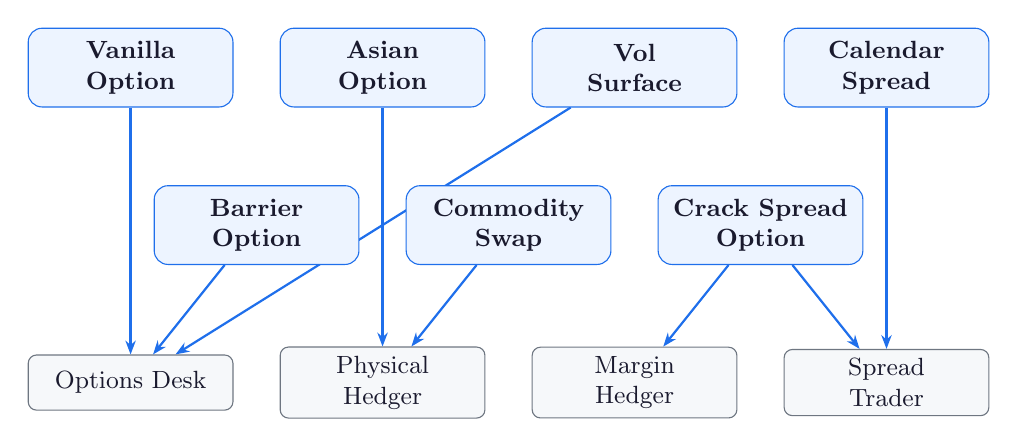
\begin{tikzpicture}[
  prod/.style={draw=accentblue,fill=boxbg,rounded corners=5pt,
               minimum width=2.6cm,minimum height=1.0cm,
               font=\small\bfseries,text=darktext,align=center},
  user/.style={draw=signalgray,fill=lightgray,rounded corners=3pt,
               minimum width=2.6cm,minimum height=0.7cm,
               font=\small,text=darktext,align=center},
  arrow/.style={-{Stealth[length=5pt]},thick,color=accentblue}
]
\node[prod] (v)   at (0,0)    {Vanilla\\Option};
\node[prod] (a)   at (3.2,0)  {Asian\\Option};
\node[prod] (c)   at (8.0,-2.0)  {Crack Spread\\Option};
\node[prod] (cal) at (9.6,0)  {Calendar\\Spread};
\node[prod] (s)   at (4.8,-2.0) {Commodity\\Swap};
\node[prod] (b)   at (1.6,-2.0){Barrier\\Option};
\node[prod] (vs)  at (6.4,0){Vol\\Surface};

\node[user] (u1) at (0,-4)   {Options Desk};
\node[user] (u2) at (3.2,-4) {Physical\\Hedger};
\node[user] (u3) at (6.4,-4) {Margin\\Hedger};
\node[user] (u4) at (9.6,-4) {Spread\\Trader};

\draw[arrow] (v)   -- (u1);
\draw[arrow] (a)   -- (u2);
\draw[arrow] (c)   -- (u4);
\draw[arrow] (c)   -- (u3);
\draw[arrow] (cal) -- (u4);
\draw[arrow] (s)   -- (u2);
\draw[arrow] (b)   -- (u1);
\begin{pgfonlayer}{background}
\draw[arrow] (vs)  -- (u1);
\end{pgfonlayer}
\end{tikzpicture}
\end{center}

\subsection{What is OCDAP?}

\textbf{OCDAP} (Options \& Commodity Derivatives Analytics Platform) is a
Python application that implements six industrial pricing engines connected
to a live forward curve downloaded from Yahoo Finance or TradingView.
It covers \textbf{65+ commodities} across 8 asset classes.

\begin{center}
\begin{tabularx}{\textwidth}{>{\bfseries}l X l}
\toprule
Tab & Product & Model \\
\midrule
Vanilla Options    & European call/put on futures                     & Black-76 \\
Asian Options      & Arithmetic/geometric average-price option         & Monte Carlo + Kemna-Vorst \\
Crack Spread       & Option on refining margin $F_2 - F_1$            & Kirk (1995) \\
Calendar Spread    & Option on curve slope $F_{\text{near}}-F_{\text{far}}$ & Kirk on term structure \\
Commodity Swaps    & Fixed-for-floating commodity swap                 & Discounted cashflows \\
Barrier Options    & Knock-in / knock-out                              & Daily Monte Carlo \\
Vol Surface        & Parametric implied volatility surface             & Black-76 + skew \\
Forward Curve      & Live futures curve + cost-of-carry extension      & Yahoo Finance / TradingView \\
\bottomrule
\end{tabularx}
\end{center}

% =============================================================================
\section{Architecture}
% =============================================================================

\subsection{The Pricing Pipeline}

\begin{center}
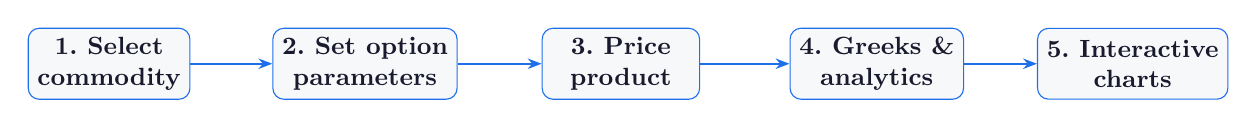
\begin{tikzpicture}[
    box/.style={draw=accentblue,fill=lightgray,rounded corners=4pt,
                minimum width=2.0cm,minimum height=0.9cm,
                font=\small\bfseries,text=darktext,align=center},
    arrow/.style={-{Stealth[length=5pt]},thick,color=accentblue}
]
\node[box] (A) at (0,0)    {1.~Select\\commodity};
\node[box] (B) at (3.25,0)  {2.~Set option\\parameters};
\node[box] (C) at (6.5,0)  {3.~Price\\product};
\node[box] (D) at (9.75,0)  {4.~Greeks \&\\analytics};
\node[box] (E) at (13.0,0) {5.~Interactive\\charts};
\draw[arrow] (A)--(B); \draw[arrow] (B)--(C);
\draw[arrow] (C)--(D); \draw[arrow] (D)--(E);
\end{tikzpicture}
\end{center}

\subsection{Expiry-Aware Ticker Generation}

A critical design choice: OCDAP always downloads the \textbf{true front month},
not an expired contract. The timeline below shows why:

\medskip
\begin{center}
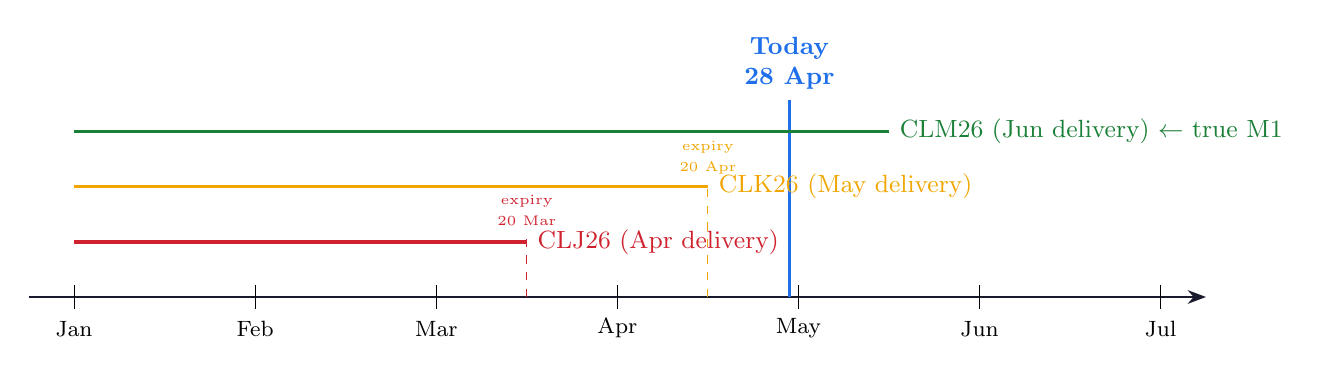
\begin{tikzpicture}[xscale=1.15]
  % Timeline axis
  \draw[-{Stealth},thick,color=darktext] (-0.5,0) -- (12.5,0);
  \foreach \x/\lbl in {0/Jan,1/Feb,2/Mar,3/Apr,4/May,5/Jun,6/Jul}{
    \draw (\x*2,0.15)--(\x*2,-0.15);
    \node[font=\footnotesize] at (\x*2,-0.4) {\lbl};
  }
  % Today marker
  \draw[very thick,color=accentblue] (7.9,0) -- (7.9,2.5)
    node[above,font=\small\bfseries,color=accentblue] {\shortstack{Today\\28 Apr}};
% Contracts
  \draw[very thick,color=signalred]  (0,0.7) -- (5,0.7)
    node[right,font=\small,color=signalred] {CLJ26 (Apr delivery)};
  \draw[very thick,color=amber]      (0,1.4) -- (7,1.4)
    node[right,font=\small,color=amber] {CLK26 (May delivery)};
  \draw[very thick,color=signalgreen](0,2.1) -- (9,2.1)
    node[right,font=\small,color=signalgreen] {CLM26 (Jun delivery) $\leftarrow$ true M1};
  % Expiry markers
  \draw[dashed,color=signalred]   (5,0) -- (5,0.79)
    node[above,font=\tiny,color=signalred] {\shortstack{expiry\\20 Mar}};
  \draw[dashed,color=amber]       (7,0) -- (7,1.44)
    node[above,font=\tiny,color=amber] {\shortstack{expiry\\20 Apr}};
  \end{tikzpicture}
\end{center}

% =============================================================================
\section{Black-76 Vanilla Option Pricer}
% =============================================================================

\subsection{Why Black-76 and Not Black-Scholes?}

\begin{center}
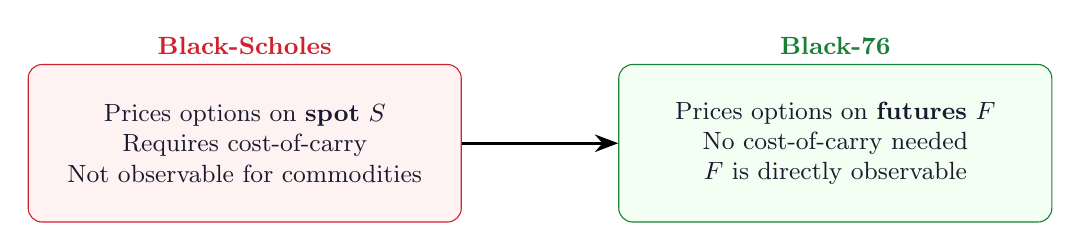
\begin{tikzpicture}
\node[draw=signalred,fill=red!5,rounded corners=5pt,
      minimum width=5.5cm,minimum height=2.0cm,
      font=\small,align=center,text=darktext,label={[font=\small\bfseries,color=signalred]above:Black-Scholes}]
  (bs) at (0,0) {\shortstack{Prices options on \textbf{spot} $S$\\Requires cost-of-carry\\Not observable for commodities}};
\node[draw=signalgreen,fill=green!5,rounded corners=5pt,
      minimum width=5.5cm,minimum height=2.0cm,
      font=\small,align=center,text=darktext,label={[font=\small\bfseries,color=signalgreen]above:Black-76}]
  (b76) at (7.5,0) {Prices options on \textbf{futures} $F$\\No cost-of-carry needed\\$F$ is directly observable};
\draw[-{Stealth},very thick,color=black] (bs) -- node[above,font=\small\bfseries]{} (b76);
\end{tikzpicture}
\end{center}

\subsection{Pricing Formula}

\begin{equation}
\boxed{C = e^{-rT}\bigl[F \cdot N(d_1) - K \cdot N(d_2)\bigr]}
\qquad
\boxed{P = e^{-rT}\bigl[K \cdot N(-d_2) - F \cdot N(-d_1)\bigr]}
\end{equation}

\[
d_1 = \frac{\ln(F/K) + \tfrac{1}{2}\sigma^2 T}{\sigma\sqrt{T}},
\qquad d_2 = d_1 - \sigma\sqrt{T}
\]

\subsection{Payoff Diagrams}

\begin{center}
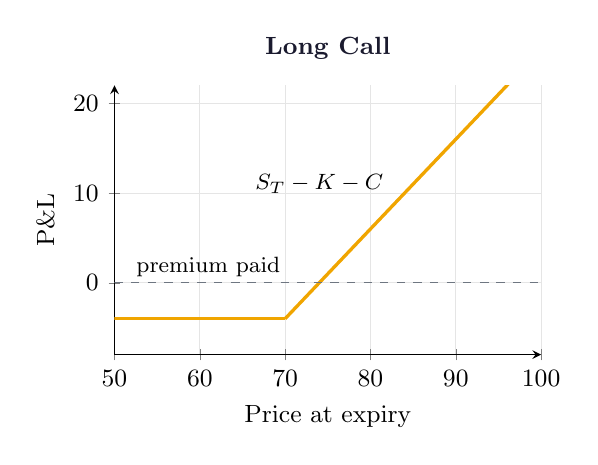
\begin{tikzpicture}
\begin{axis}[
    width=7cm,height=5cm,
    xlabel={Price at expiry},ylabel={P\&L},
    xmin=50,xmax=100,ymin=-8,ymax=22,
    grid=both,grid style={draw=gray!20},
    axis lines=left,tick label style={font=\small},
    label style={font=\small},
    title={\small\bfseries Long Call},
    title style={color=darktext}
]
\addplot[color=amber,very thick,domain=50:70] {-4};
\addplot[color=amber,very thick,domain=70:100] {x-74};
\addplot[dashed,color=signalgray,domain=50:100] {0};
\node[font=\footnotesize] at (axis cs:61,1.8) {premium paid};
\node[font=\footnotesize] at (axis cs:74,11) {$S_T - K - C$};
\end{axis}
\end{tikzpicture}
\hspace{1cm}
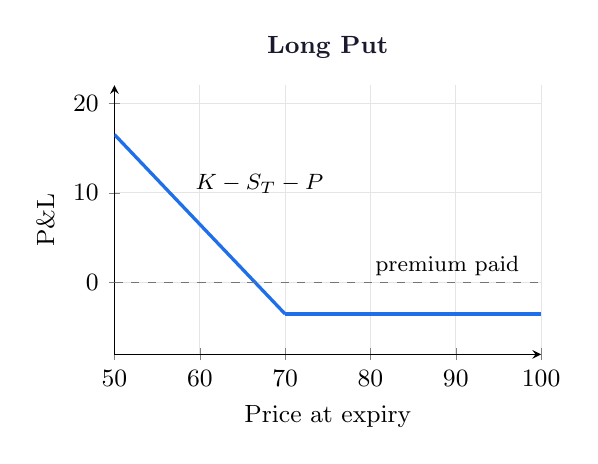
\begin{tikzpicture}
\begin{axis}[
    width=7cm,height=5cm,
    xlabel={Price at expiry},ylabel={P\&L},
    xmin=50,xmax=100,ymin=-8,ymax=22,
    grid=both,grid style={draw=gray!20},
    axis lines=left,tick label style={font=\small},
    label style={font=\small},
    title={\small\bfseries Long Put},
    title style={color=darktext}
]
\addplot[color=accentblue,very thick,domain=70:100] {-3.5};
\addplot[color=accentblue,very thick,domain=50:70]  {66.5-x};
\addplot[dashed,color=signalgray,domain=50:100] {0};
\node[font=\footnotesize] at (axis cs:89,1.8) {premium paid};
\node[font=\footnotesize] at (axis cs:67,11) {$K - S_T - P$};
\end{axis}
\end{tikzpicture}
\end{center}

\subsection{Greeks}

{\renewcommand{\arraystretch}{3}
\begin{center}
\begin{tabularx}{\textwidth}{c c X}
\toprule
Greek & Formula (call) & Economic interpretation \\
\midrule
$\Delta$ & $e^{-rT} N(d_1)$ & Futures equivalent: how many futures to hold to delta-hedge \\
$\Gamma$ & $\dfrac{e^{-rT} N'(d_1)}{F\sigma\sqrt{T}}$ & Rate of change of delta --- cost of dynamic rebalancing \\
$\mathcal{V}$ & $\dfrac{e^{-rT} F N'(d_1)\sqrt{T}}{100}$ & P\&L per 1\% implied vol move \\
$\Theta$ & $\dfrac{-e^{-rT}F N'(d_1)\sigma}{2\sqrt{T}\cdot 365}$ & Daily time decay (negative for long options) \\
$\rho$ & $\dfrac{-Te^{-rT}(FN(d_1)-KN(d_2))}{100}$ & Sensitivity to risk-free rate per 1\% \\
\bottomrule
\end{tabularx}
\end{center}}

\subsection{Put-Call Parity}

\begin{equation}
C - P = e^{-rT}(F - K)
\end{equation}

OCDAP verifies this numerically for every pair. The typical numerical error is
below $10^{-4}$, displayed as \texttt{\checkmark\ verified} in the dashboard.

% =============================================================================
\section{Asian Option Pricer}
% =============================================================================

\subsection{Why Asian Options in Commodity Markets?}

\begin{center}
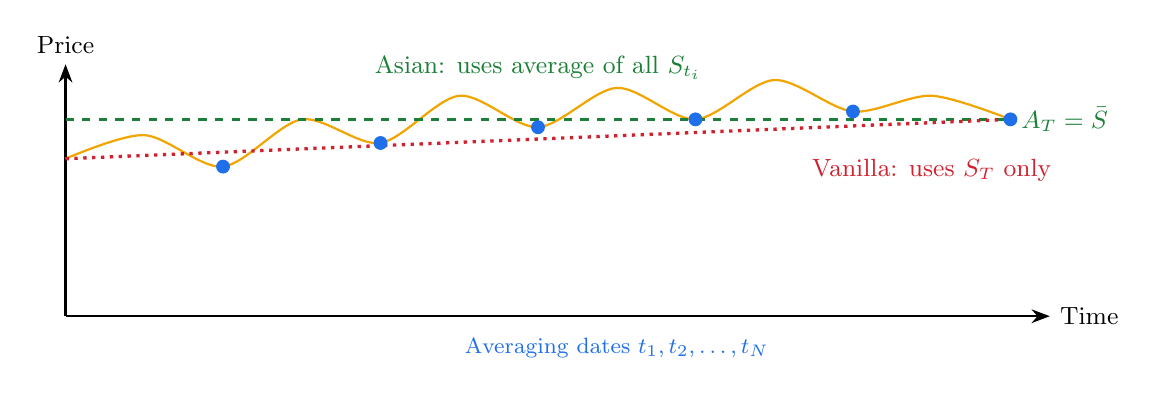
\begin{tikzpicture}[xscale=1.0]
  \draw[-{Stealth},thick] (0,0) -- (12.5,0) node[right,font=\small] {Time};
  \draw[-{Stealth},thick] (0,0) -- (0,3.2) node[above,font=\small] {Price};
  % Simulated path
  \draw[color=amber,thick,smooth] plot coordinates
    {(0,2.0)(1,2.3)(2,1.9)(3,2.5)(4,2.2)(5,2.8)
     (6,2.4)(7,2.9)(8,2.5)(9,3.0)(10,2.6)(11,2.8)(12,2.5)};
  % Average line
  \draw[color=signalgreen,very thick,dashed] (0,2.5) -- (12,2.5)
    node[right,font=\small,color=signalgreen] {$A_T = \bar{S}$};
  % Vanilla payoff line
  \draw[color=signalred,very thick,dotted] (0,2.0) -- (12,2.5);
  \node[color=signalred,font=\small] at (11,1.85) {Vanilla: uses $S_T$ only};
  \node[color=signalgreen,font=\small] at (6,3.15) {Asian: uses average of all $S_{t_i}$};
  % Observation dots
  \foreach \x/\y in {2/1.9,4/2.2,6/2.4,8/2.5,10/2.6,12/2.5}{
    \fill[color=accentblue] (\x,\y) circle (2.5pt);
  }
  \node[font=\footnotesize,color=accentblue] at (7,-0.4) {Averaging dates $t_1, t_2, \ldots, t_N$};
\end{tikzpicture}
\end{center}

\subsection{Monte Carlo Simulation}

Under the risk-neutral measure, futures prices follow GBM with zero drift:

\begin{equation}
S_{t+\Delta t} = S_t \cdot \exp\!\left(-\tfrac{1}{2}\sigma^2\Delta t + \sigma\sqrt{\Delta t}\,Z\right),
\quad Z \sim \mathcal{N}(0,1)
\end{equation}

\begin{equation}
C_{\text{Asian}} = e^{-rT} \cdot \frac{1}{M}\sum_{j=1}^{M}\max\!\left(\frac{1}{N}\sum_{i=1}^{N}S_{t_i}^{(j)} - K,\;0\right)
\end{equation}

\subsection{Arithmetic vs.\ Geometric Average}

\begin{center}
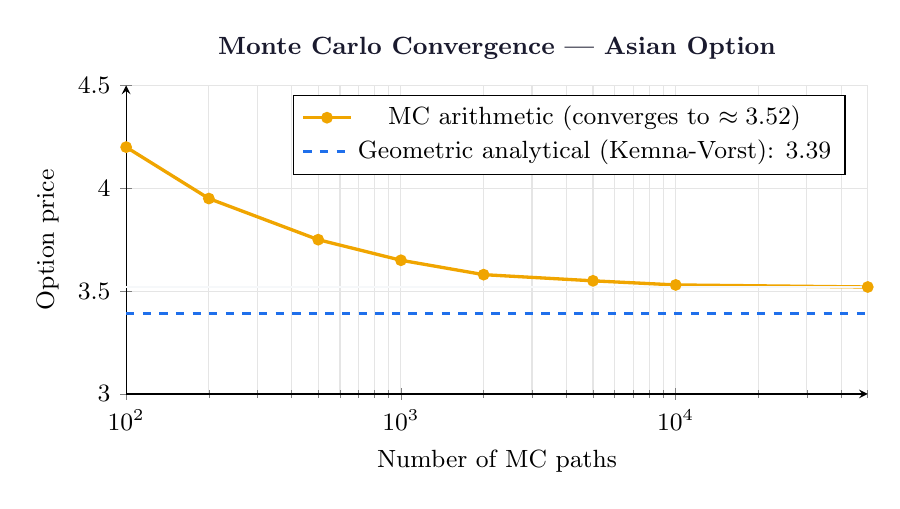
\begin{tikzpicture}
\begin{axis}[
    width=11cm,height=5.5cm,
    xlabel={Number of MC paths},
    ylabel={Option price},
    xmode=log,
    xmin=100,xmax=50000,
    ymin=3.0,ymax=4.5,
    grid=both,grid style={draw=gray!20},
    axis lines=left,
    tick label style={font=\small},
    label style={font=\small},
    legend style={font=\small,at={(0.97,0.97)},anchor=north east},
    title={\small\bfseries Monte Carlo Convergence --- Asian Option},
    title style={color=darktext}
]
% Simulated convergence (illustrative)
\addplot[color=amber,very thick,mark=*,mark size=1.5pt] coordinates
  {(100,4.20)(200,3.95)(500,3.75)(1000,3.65)(2000,3.58)(5000,3.55)(10000,3.53)(50000,3.52)};
\addlegendentry{MC arithmetic (converges to $\approx 3.52$)}
\addplot[color=accentblue,very thick,dashed] coordinates
  {(100,3.39)(50000,3.39)};
\addlegendentry{Geometric analytical (Kemna-Vorst): 3.39}
\addplot[color=lightgray,thin] coordinates {(100,3.52)(50000,3.52)};
\end{axis}
\end{tikzpicture}
\end{center}

\begin{notebox}
\textbf{Ordering property (AM-GM inequality):} The arithmetic average always exceeds
or equals the geometric average. Therefore, the arithmetic Asian call is always
\textit{at least as expensive} as the Kemna-Vorst geometric price. OCDAP verifies
this automatically as a sanity check.
\end{notebox}

\subsection{Geometric Average --- Kemna-Vorst (1990)}

\begin{equation}
\sigma_g = \sigma\sqrt{\frac{2N+1}{6(N+1)}}, \qquad b_g = \frac{1}{2}\!\left(-\frac{\sigma^2}{6} + \sigma_g^2\right), \qquad F_g = F\cdot e^{b_g T}
\end{equation}

% =============================================================================
\section{Crack Spread Option Pricer}
% =============================================================================

\subsection{The Refining Margin}

\begin{center}
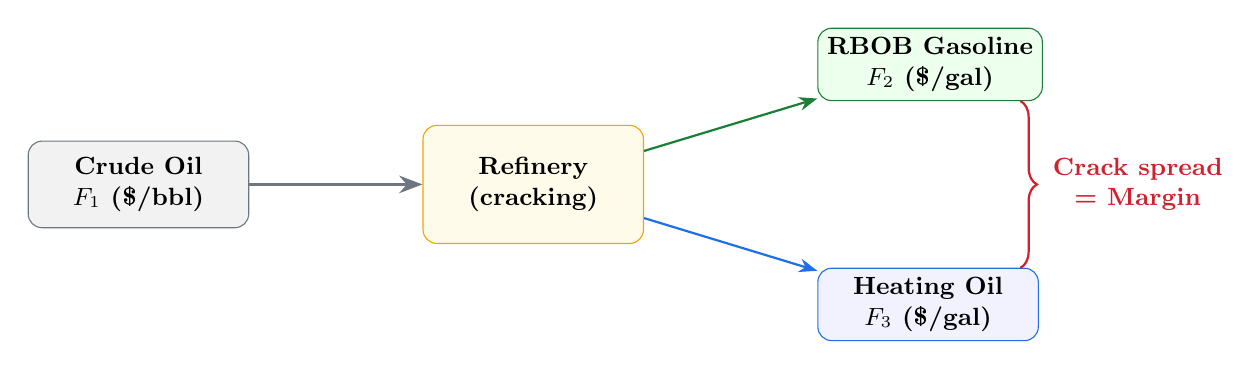
\begin{tikzpicture}[node distance=1.4cm]
  \node[draw=signalgray,fill=gray!10,rounded corners=5pt,
        minimum width=2.8cm,minimum height=1.1cm,
        font=\small\bfseries,align=center] (crude)
    {Crude Oil\\$F_1$ (\$/bbl)};
  \node[draw=amber,fill=notebg,rounded corners=5pt,
        minimum width=2.8cm,minimum height=1.5cm,
        font=\small\bfseries,align=center,right=2.2cm of crude] (refinery)
    {Refinery\\(cracking)};
  \node[draw=signalgreen,fill=green!7,rounded corners=5pt,
        minimum width=2.8cm,minimum height=0.9cm,
        font=\small\bfseries,align=center,above right=0.3cm and 2.2cm of refinery] (rbob)
    {RBOB Gasoline\\$F_2$ (\$/gal)};
  \node[draw=accentblue,fill=blue!5,rounded corners=5pt,
        minimum width=2.8cm,minimum height=0.9cm,
        font=\small\bfseries,align=center,below right=0.3cm and 2.2cm of refinery] (ho)
    {Heating Oil\\$F_3$ (\$/gal)};
  \draw[-{Stealth},very thick,color=signalgray] (crude) -- (refinery);
  \draw[-{Stealth},thick,color=signalgreen] (refinery) -- (rbob);
  \draw[-{Stealth},thick,color=accentblue] (refinery) -- (ho);
  % Crack spread brace
  \draw[decorate,decoration={brace,amplitude=6pt},color=signalred,thick]
    (11.2,1.06) -- (11.2,-1.06)
    node[midway,right=8pt,font=\small\bfseries,color=signalred] {\shortstack{Crack spread\\= Margin}};
\end{tikzpicture}
\end{center}

\[
\text{3-2-1 Crack} = \tfrac{1}{3}\bigl(2\cdot F_{\text{RBOB}}\cdot 42 + F_{\text{HO}}\cdot 42\bigr) - F_{\text{WTI}}
\]

\subsection{Kirk (1995) Approximation}

\begin{equation}
\alpha = \frac{F_2}{F_2 + Ke^{-rT}},
\qquad
\boxed{\sigma_{\text{Kirk}} = \sqrt{\sigma_1^2 + (\alpha\sigma_2)^2 - 2\rho\,\sigma_1\sigma_2\,\alpha}}
\end{equation}

\begin{center}
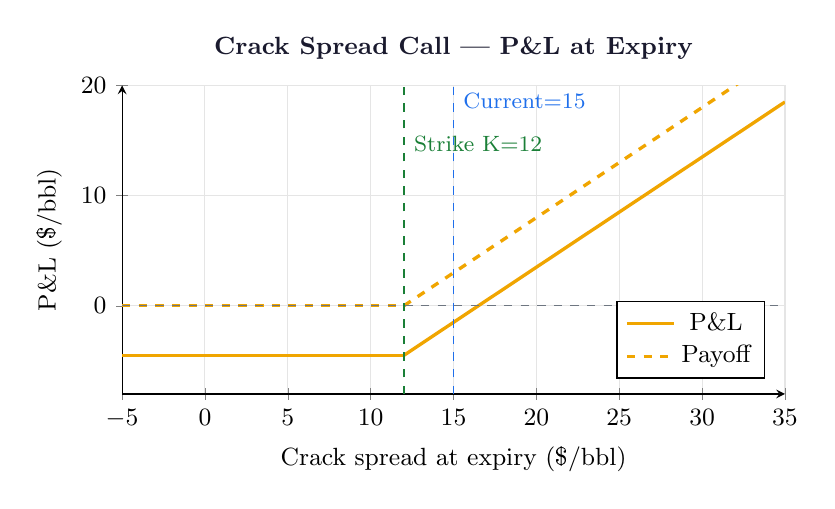
\begin{tikzpicture}
\begin{axis}[
    width=10cm,height=5.5cm,
    xlabel={Crack spread at expiry (\$/bbl)},
    ylabel={P\&L (\$/bbl)},
    xmin=-5,xmax=35,
    ymin=-8,ymax=20,
    grid=both,grid style={draw=gray!20},
    axis lines=left,
    tick label style={font=\small},
    label style={font=\small},
    legend style={font=\small,at={(0.97,0.05)},anchor=south east},
    title={\small\bfseries Crack Spread Call --- P\&L at Expiry},
    title style={color=darktext}
]
\addplot[color=amber,very thick,domain=-5:12] {-4.5};
\addplot[color=amber,very thick,dashed,domain=-5:12]   {0};
\addplot[color=amber,very thick,domain=12:35]  {x-16.5};
\addplot[color=amber,very thick,dashed,domain=12:35]   {x-12};
\addplot[dashed,color=signalgray,domain=-5:35] {0};
\draw[dashed,color=signalgreen,thick] (axis cs:12,-8) -- (axis cs:12,20)
  node[pos=0.81, right,font=\footnotesize,color=signalgreen] {Strike K=12};
\draw[dashed,color=accentblue,thin] (axis cs:15,-8) -- (axis cs:15,20)
  node[pos=0.95, right,font=\footnotesize,color=accentblue] {Current=15};
\addlegendentry{P\&L}
\addlegendentry{Payoff}
\end{axis}
\end{tikzpicture}
\end{center}

% =============================================================================
\section{Calendar Spread Option Pricer}
% =============================================================================

\subsection{What a Calendar Spread Option Trades}

\begin{center}
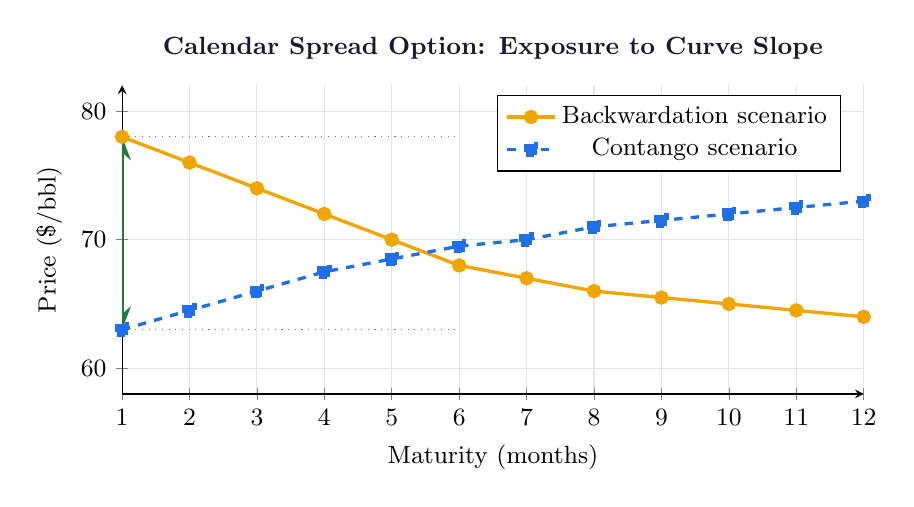
\begin{tikzpicture}
\begin{axis}[
    width=11cm,height=5.5cm,
    xlabel={Maturity (months)},
    ylabel={Price (\$/bbl)},
    xmin=1,xmax=12,
    ymin=58,ymax=82,
    grid=both,grid style={draw=gray!20},
    axis lines=left,
    tick label style={font=\small},
    label style={font=\small},
    xtick={1,2,3,4,5,6,7,8,9,10,11,12},
    legend style={font=\small,at={(0.97,0.97)},anchor=north east},
    title={\small\bfseries Calendar Spread Option: Exposure to Curve Slope},
    title style={color=darktext}
]
\addplot[color=amber,very thick,mark=*,mark size=2pt] coordinates
  {(1,78)(2,76)(3,74)(4,72)(5,70)(6,68)(7,67)(8,66)(9,65.5)(10,65)(11,64.5)(12,64)};
\addlegendentry{Backwardation scenario}
\addplot[color=accentblue,very thick,mark=square*,mark size=2pt,dashed] coordinates
  {(1,63)(2,64.5)(3,66)(4,67.5)(5,68.5)(6,69.5)(7,70)(8,71)(9,71.5)(10,72)(11,72.5)(12,73)};
\addlegendentry{Contango scenario}
% Brace for M1-M6 spread
\draw[{Stealth}-{Stealth},very thick,color=signalgreen]
  (axis cs:1,78) -- (axis cs:1,63)
  node[midway,left=4pt,font=\small\bfseries,color=signalgreen] {M1-M6 spread};
\draw[dotted,color=signalgray] (axis cs:1,63) -- (axis cs:6,63);
\draw[dotted,color=signalgray] (axis cs:1,78) -- (axis cs:6,78);
\end{axis}
\end{tikzpicture}
\end{center}

\subsection{Kirk on the Term Structure}

\begin{equation}
\alpha = \frac{F_{\text{near}}}{F_{\text{near}} + Ke^{-rT}},
\qquad
\sigma_{\text{Kirk}} = \sqrt{\sigma_{\text{far}}^2 + (\alpha\,\sigma_{\text{near}})^2 - 2\rho\,\sigma_{\text{far}}\,\sigma_{\text{near}}\,\alpha}
\end{equation}

Correlation between near and far contracts is typically $\rho \in [0.90, 0.99]$.

% =============================================================================
\section{Commodity Swap Pricer}
% =============================================================================

\subsection{Cash Flow Structure}

\begin{center}
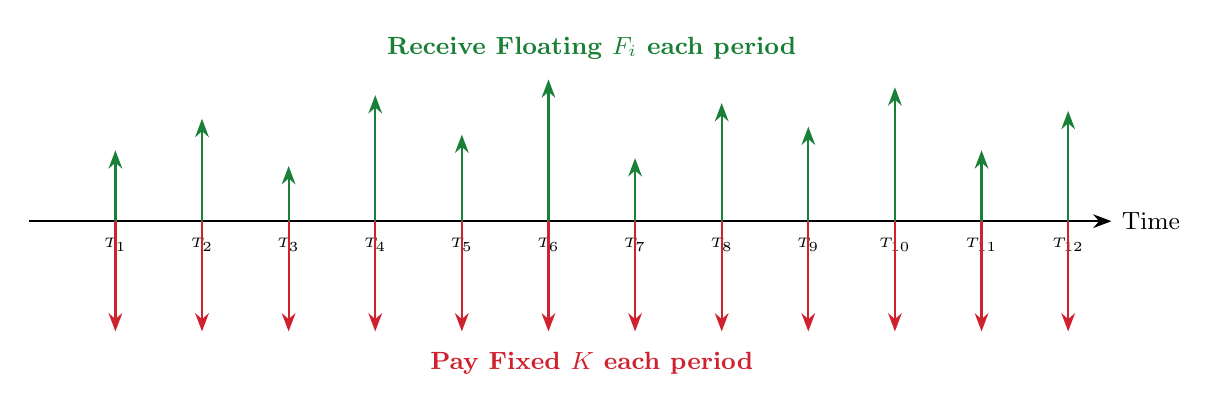
\begin{tikzpicture}[xscale=1.1]
  \draw[-{Stealth},thick] (0,0) -- (12.5,0) node[right,font=\small] {Time};
  \foreach \t in {1,2,3,4,5,6,7,8,9,10,11,12}{
    \draw (\t,0.1)--(\t,-0.1);
    \node[font=\tiny] at (\t,-0.3) {$T_{\t}$};
  }
  % Fixed payments (down)
  \foreach \t/\h in {1/1.4,2/1.4,3/1.4,4/1.4,5/1.4,6/1.4,7/1.4,8/1.4,9/1.4,10/1.4,11/1.4,12/1.4}{
    \draw[-{Stealth},thick,color=signalred] (\t,0) -- (\t,-\h);
  }
  \node[color=signalred,font=\small\bfseries] at (6.5,-1.8) {Pay Fixed $K$ each period};
  % Floating receipts (up, varying)
  \foreach \t/\h in {1/0.9,2/1.3,3/0.7,4/1.6,5/1.1,6/1.8,7/0.8,8/1.5,9/1.2,10/1.7,11/0.9,12/1.4}{
    \draw[-{Stealth},thick,color=signalgreen] (\t,0) -- (\t,\h);
  }
  \node[color=signalgreen,font=\small\bfseries] at (6.5,2.2) {Receive Floating $F_i$ each period};
\end{tikzpicture}
\end{center}

\begin{equation}
\boxed{\text{NPV} = \sum_{i=1}^{N} e^{-rT_i}(F_i - K)\cdot\text{notional}}
\qquad
K^* = \frac{\sum_{i=1}^{N} e^{-rT_i}\,F_i}{\sum_{i=1}^{N} e^{-rT_i}}
\end{equation}

\subsection{NPV Sensitivity to Forward Curve Shift}

\begin{center}
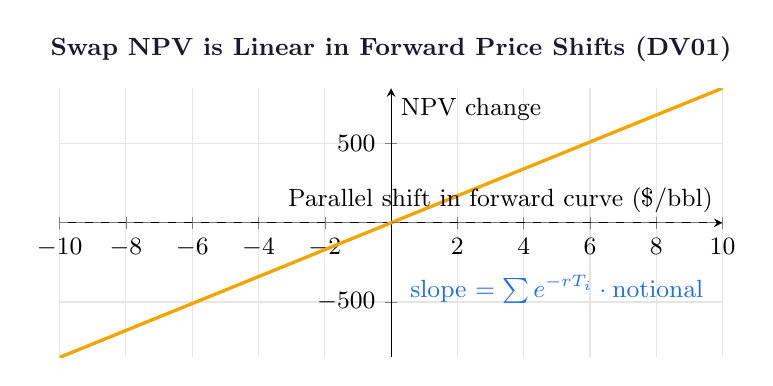
\begin{tikzpicture}
\begin{axis}[
    width=10cm,height=5cm,
    xlabel={Parallel shift in forward curve (\$/bbl)},
    ylabel={NPV change},
    xmin=-10,xmax=10,
    grid=both,grid style={draw=gray!20},
    axis lines=center,
    tick label style={font=\small},
    label style={font=\small},
    title={\small\bfseries Swap NPV is Linear in Forward Price Shifts (DV01)},
    title style={color=darktext}
]
\addplot[color=amber,very thick,domain=-10:10] {x*85};
\addplot[dashed,color=signalgray,domain=-10:10] {0};
\node[font=\small,color=accentblue] at (axis cs:5,-420)
  {slope $= \sum e^{-rT_i}\cdot\text{notional}$};
\end{axis}
\end{tikzpicture}
\end{center}

% =============================================================================
\section{Barrier Option Pricer}
% =============================================================================

\subsection{Barrier Types}

\begin{center}
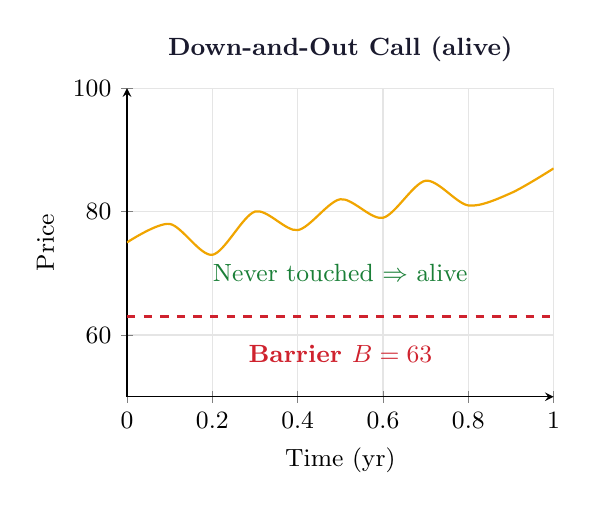
\begin{tikzpicture}
\begin{axis}[
    width=7cm,height=5.5cm,
    xlabel={Time (yr)},ylabel={Price},
    xmin=0,xmax=1,ymin=50,ymax=100,
    grid=both,grid style={draw=gray!20},
    axis lines=left,
    tick label style={font=\small},
    label style={font=\small},
    title={\small\bfseries Down-and-Out Call (alive)},
    title style={color=darktext}
]
\addplot[color=amber,thick,smooth] coordinates
  {(0,75)(0.1,78)(0.2,73)(0.3,80)(0.4,77)(0.5,82)(0.6,79)(0.7,85)(0.8,81)(0.9,83)(1.0,87)};
\addplot[very thick,dashed,color=signalred,domain=0:1] {63};
\node[color=signalred,font=\small\bfseries] at (axis cs:0.5,57) {Barrier $B=63$};
\node[color=signalgreen,font=\small] at (axis cs:0.5,70) {Never touched $\Rightarrow$ alive};
\end{axis}
\end{tikzpicture}
\hspace{0.5cm}
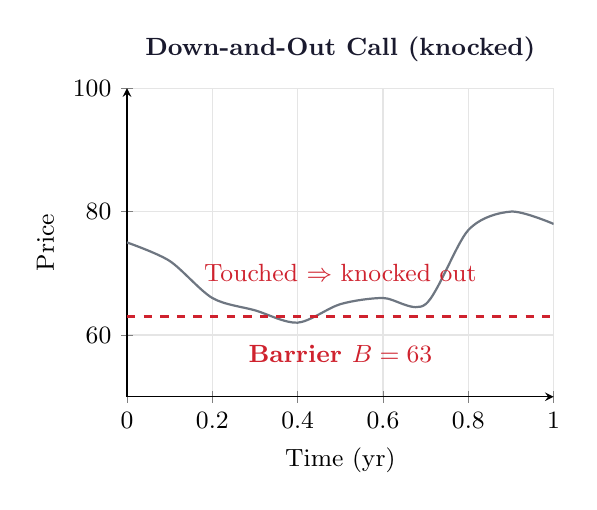
\begin{tikzpicture}
\begin{axis}[
    width=7cm,height=5.5cm,
    xlabel={Time (yr)},ylabel={Price},
    xmin=0,xmax=1,ymin=50,ymax=100,
    grid=both,grid style={draw=gray!20},
    axis lines=left,
    tick label style={font=\small},
    label style={font=\small},
    title={\small\bfseries Down-and-Out Call (knocked)},
    title style={color=darktext}
]
\addplot[color=signalgray,thick,smooth] coordinates
  {(0,75)(0.1,72)(0.2,66)(0.3,64)(0.4,62)(0.5,65)(0.6,66)(0.7,65)(0.8,77)(0.9,80)(1.0,78)};
\addplot[very thick,dashed,color=signalred,domain=0:1] {63};
\node[color=signalred,font=\small\bfseries] at (axis cs:0.5,57) {Barrier $B=63$};
\node[color=signalred,font=\small] at (axis cs:0.5,70) {Touched $\Rightarrow$ knocked out};
\end{axis}
\end{tikzpicture}
\end{center}

\subsection{Knock Probability and Discount vs Vanilla}

\begin{center}
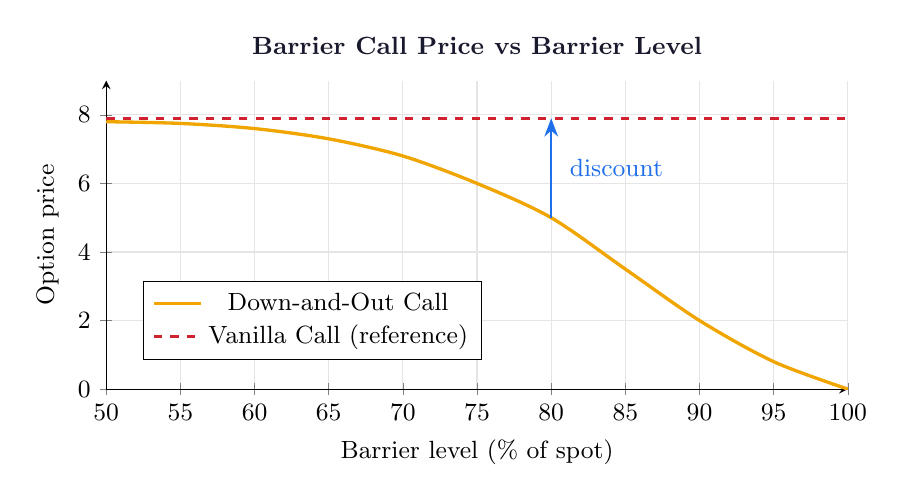
\begin{tikzpicture}
\begin{axis}[
    width=11cm,height=5.5cm,
    xlabel={Barrier level (\% of spot)},
    ylabel={Option price},
    xmin=50,xmax=100,ymin=0,ymax=9,
    grid=both,grid style={draw=gray!20},
    axis lines=left,
    tick label style={font=\small},
    label style={font=\small},
    legend style={font=\small,at={(0.05,0.35)},anchor=north west},
    title={\small\bfseries Barrier Call Price vs Barrier Level},
    title style={color=darktext}
]
\addplot[color=amber,very thick,smooth] coordinates
  {(50,7.8)(55,7.75)(60,7.6)(65,7.3)(70,6.8)(75,6.0)(80,5.0)(85,3.5)(90,2.0)(95,0.8)(100,0)};
\addplot[color=signalred,very thick,dashed,domain=50:100] {7.9};
\addlegendentry{Down-and-Out Call}
\addlegendentry{Vanilla Call (reference)}
\draw[-{Stealth},color=accentblue,thick]
  (axis cs:80,5.0) -- (axis cs:80,7.9)
  node[midway,right=3pt,font=\small,color=accentblue] {discount};
\end{axis}
\end{tikzpicture}
\end{center}

% =============================================================================
\section{Volatility Surface}
% =============================================================================

\subsection{The Smile and Skew}

\begin{center}
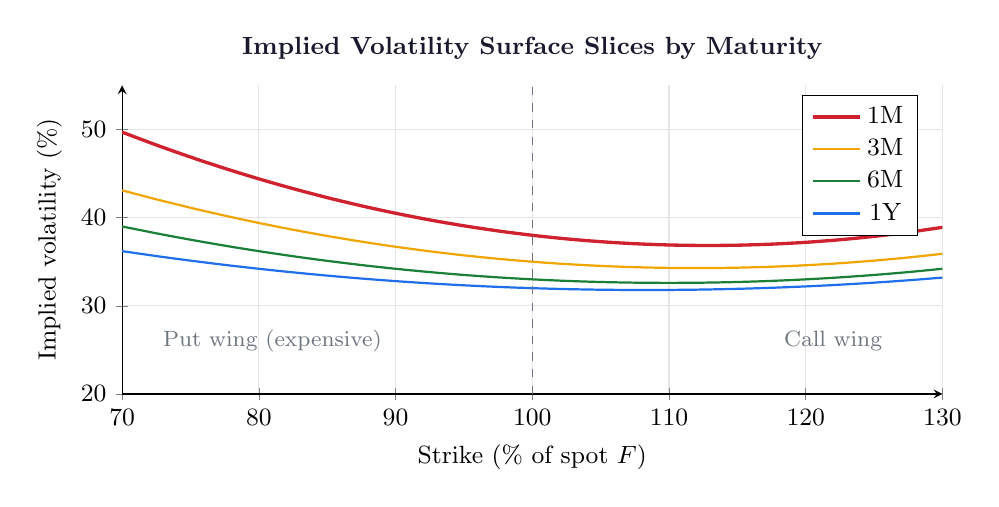
\begin{tikzpicture}
\begin{axis}[
    width=12cm,height=5.5cm,
    xlabel={Strike (\% of spot $F$)},
    ylabel={Implied volatility (\%)},
    xmin=70,xmax=130,
    ymin=20,ymax=55,
    grid=both,grid style={draw=gray!20},
    axis lines=left,
    tick label style={font=\small},
    label style={font=\small},
    legend style={font=\small,at={(0.97,0.97)},anchor=north east},
    title={\small\bfseries Implied Volatility Surface Slices by Maturity},
    title style={color=darktext}
    ]
% 1M smile (steepest)
\addplot[color=signalred,very thick,smooth,domain=70:130]
  {38 - 0.18*(x-100) + 0.007*(x-100)^2};
\addlegendentry{1M}
% 3M
\addplot[color=amber,thick,smooth,domain=70:130]
  {35 - 0.12*(x-100) + 0.005*(x-100)^2};
\addlegendentry{3M}
% 6M
\addplot[color=signalgreen,thick,smooth,domain=70:130]
  {33 - 0.08*(x-100) + 0.004*(x-100)^2};
\addlegendentry{6M}
% 1Y (flattest)
\addplot[color=accentblue,thick,smooth,domain=70:130]
  {32 - 0.05*(x-100) + 0.003*(x-100)^2};
\addlegendentry{1Y}
% ATM marker
\draw[dashed,color=signalgray] (axis cs:100,20) -- (axis cs:100,55)
  node[above,font=\small] {ATM};
\node[font=\footnotesize,color=signalgray] at (axis cs:81,26)
  {Put wing (expensive)};
\node[font=\footnotesize,color=signalgray] at (axis cs:122,26)
  {Call wing};
\end{axis}
\end{tikzpicture}
\end{center}

\subsection{Parametric Model}

\begin{equation}
\sigma(K,T) = \underbrace{\sigma_{\text{ATM}}\!(1+\nu\sqrt{T})}_{\text{ATM term structure}}
+ \underbrace{\text{skew}\cdot\ln\!\tfrac{K}{F}}_{\text{slope}}
+ \underbrace{\text{curvature}\cdot\!\left(\ln\!\tfrac{K}{F}\right)^2}_{\text{wings}}
\end{equation}

\begin{center}
\begin{tabularx}{\textwidth}{>{\bfseries}l X l}
\toprule
Parameter & Economic meaning & WTI typical \\
\midrule
ATM vol $\sigma$ & Base vol at the money & 30\% \\
Skew & Puts expensive relative to calls. Negative in most commodity markets. & $-0.03$ \\
Curvature & How quickly vol rises in the wings. Positive = symmetric smile. & $+0.05$ \\
Steepness $\nu$ & Term structure slope. Short-dated vol $>$ long-dated vol. & $+0.08$ \\
\bottomrule
\end{tabularx}
\end{center}

% =============================================================================
\section{Forward Curve Data Layer}
% =============================================================================

\subsection{Cost-of-Carry Model}

\begin{equation}
F(T) = S \cdot e^{(r + u - cy)\,T}
\end{equation}

\begin{center}
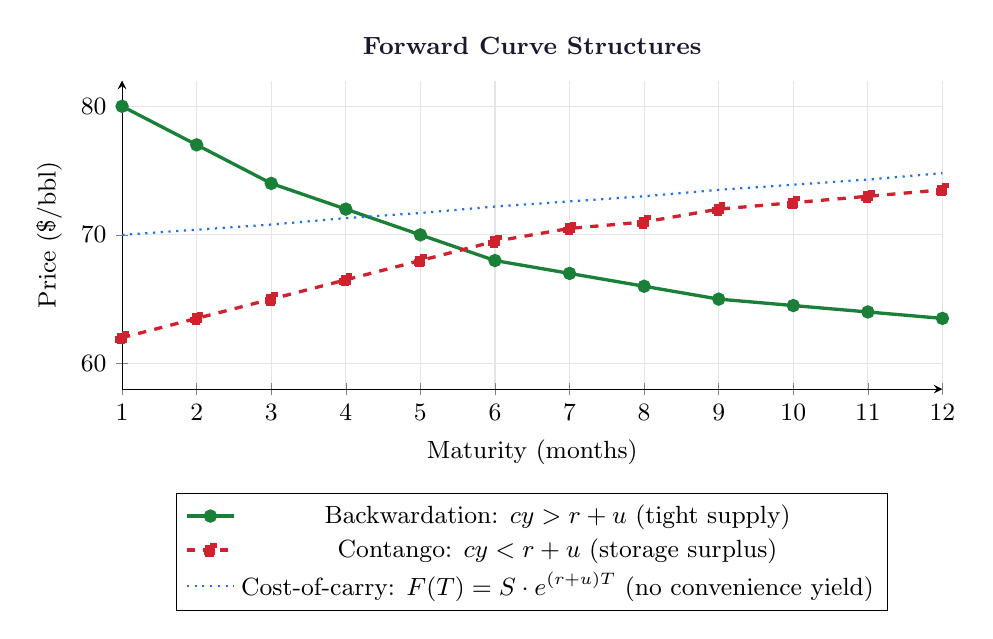
\begin{tikzpicture}
\begin{axis}[
    width=12cm,height=5.5cm,
    xlabel={Maturity (months)},
    ylabel={Price (\$/bbl)},
    xmin=1,xmax=12,
    ymin=58,ymax=82,
    xtick={1,2,3,4,5,6,7,8,9,10,11,12},
    grid=both,grid style={draw=gray!20},
    axis lines=left,
    tick label style={font=\small},
    label style={font=\small},
    legend style={font=\small,at={(0.5,-0.72)},anchor=south},
    title={\small\bfseries Forward Curve Structures},
    title style={color=darktext}
]
\addplot[color=signalgreen,very thick,mark=*,mark size=1.8pt] coordinates
  {(1,80)(2,77)(3,74)(4,72)(5,70)(6,68)(7,67)(8,66)(9,65)(10,64.5)(11,64)(12,63.5)};
\addlegendentry{Backwardation: $cy > r+u$ (tight supply)}
\addplot[color=signalred,very thick,mark=square*,mark size=1.8pt,dashed] coordinates
  {(1,62)(2,63.5)(3,65)(4,66.5)(5,68)(6,69.5)(7,70.5)(8,71)(9,72)(10,72.5)(11,73)(12,73.5)};
\addlegendentry{Contango: $cy < r+u$ (storage surplus)}
\addplot[color=accentblue,thick,dotted] coordinates
  {(1,70)(2,70.4)(3,70.8)(4,71.3)(5,71.7)(6,72.2)(7,72.6)(8,73)(9,73.5)(10,73.9)(11,74.3)(12,74.8)};
\addlegendentry{Cost-of-carry: $F(T) = S\cdot e^{(r+u)T}$ (no convenience yield)}
\end{axis}
\end{tikzpicture}
\end{center}

% =============================================================================
\section{Potential Applications and Extensions}
% =============================================================================

\begin{center}
\begin{tabularx}{\textwidth}{>{\bfseries}l X}
\toprule
User & How OCDAP helps \\
\midrule
Airline treasurer
  & Price Asian calls on jet fuel based on monthly average procurement cost.
    Compare vanilla vs barrier option premium to reduce hedging cost. \\
Crude oil refiner
  & Price 3-2-1 crack spread options to protect gross refining margin.
    Use commodity swaps to lock in a fixed crude purchase price for 12 months. \\
Commodity trader
  & Price calendar spread options to speculate on steepening or flattening.
    Use the vol surface to assess whether implied vol is rich or cheap
    relative to ATM. \\
Risk manager
  & Compute DV01 and cashflow sensitivity for swap portfolios.
    Quantify knock-out probability and discount on barrier options. \\
Student / practitioner
  & Apply six pricing engines to 65+ commodities with live data.
    All formulas, models and assumptions are transparent and documented. \\
\bottomrule
\end{tabularx}
\end{center}

\subsection{Possible Quantitative Extensions}

\textbf{Implied volatility surface from real option chains.}
Yahoo Finance exposes option chain data for liquid futures (WTI, Gold, Corn)
via \texttt{yfinance}. OCDAP could extract real market-implied vols per strike
and maturity, and overlay them against the parametric model to reveal the smile
or skew actually priced by the market.

\textbf{Stochastic volatility (SABR model).}
The SABR model is the industry standard for capturing the volatility smile in
interest rate and commodity derivatives. Replacing the flat-vol Black-76 pricer
with SABR would produce more realistic prices for OTM options.

\textbf{Swing options.}
Swing options are standard in European gas and power markets. They give the holder
the right to take or deliver gas at a variable daily volume within contractual bounds.
Pricing requires dynamic programming and is directly applicable to Engie, TotalEnergies,
and EDF trading desks.

\textbf{Monte Carlo Schwartz-Smith simulation.}
Using the SS calibrated parameters $(\kappa, \xi_0, \sigma_\chi, \sigma_\xi)$ as
diffusion inputs, OCDAP could simulate full paths of the futures curve and price
path-dependent exotic options (barrier, Asian, lookback) in a single consistent framework.

% =============================================================================
\section{Conclusion}
% =============================================================================

OCDAP demonstrates how a professional-grade commodity derivatives pricer can
be built entirely in Python with freely available market data.

Six pricing engines cover the full spectrum of products used by commodity desks:
vanilla options (Black-76), average-price options (Monte Carlo), spread options
(Kirk 1995), curve slope options, fixed-for-floating swaps, and path-dependent
barriers. The expiry-aware ticker logic ensures prices are always sourced from
live, non-expired futures contracts.

Together with CFCAP, OCDAP provides a complete analytical stack for the
commodity markets: curve analysis and signals on one side, derivatives pricing
and risk on the other.


\end{document}
